\documentclass[a4paper, zihao=-4, UTF-8]{ctexart}
\usepackage{graphicx}
\usepackage{subfigure}
\usepackage{caption2}


\renewcommand{\figurename}{图}
\renewcommand{\captionlabeldelim}{.}
\renewcommand{\thesubfigure} {\thefigure.\arabic{subfigure}} \makeatletter
\renewcommand{\@thesubfigure}{\thesubfigure:\space} \renewcommand{\p@subfigure}{} \makeatother
\renewcommand{\tablename}{表}

\usepackage{enumerate}

\usepackage {ctex}
\usepackage{hyperref}
\hypersetup{
	colorlinks=true,
	citecolor=black,
	linkcolor=black
}

\usepackage{geometry}
\geometry{a4paper,left=2.5cm,right=2.5cm,top=2.5cm,bottom=2.5cm}
\setlength{\parindent}{2em}
\setmonofont{Consolas}
\setsansfont{Consolas}
\setmainfont{Times New Roman}

\usepackage{fancyhdr}
\pagestyle{fancy}
\renewcommand{\headrulewidth}{0pt}

\usepackage{authblk}
\renewcommand*{\Affilfont}{\small} % 修改机构名称的字体与大小
\renewcommand\Authand{, } % 去掉 and 前的逗号

\usepackage{indentfirst}
\setlength{\parindent}{2em}

\usepackage{amsmath}
\usepackage{amssymb}
\CTEXsetup[format={\Large\bfseries}]{section}
\usepackage{xcolor}
\usepackage{listings}
\renewcommand{\lstlistingname}{代码}
\lstset{
	columns=fixed,
	breakatwhitespace=true,
	breaklines=true,
	breakindent=26pt,
	captionpos=bl,
	numbers=left,
	frame=shadowbox,
	basicstyle=\ttfamily,
	keywordstyle=\ttfamily\color{blue},
	numberstyle=\footnotesize\color{darkgray},
	commentstyle=\ttfamily\it\color[RGB]{0,96,96},
	stringstyle=\ttfamily\color{magenta},
	showstringspaces=false,
	language=Python,
	identifierstyle=\ttfamily,
	tabsize=4,
}

\usepackage{algorithm}
\usepackage{algorithmicx}
\usepackage{algpseudocode}
\renewcommand{\algorithmicrequire}{\textbf{Input:}}  % Use Input in the format of Algorithm  
\renewcommand{\algorithmicensure}{\textbf{Output:}} % Use Output in the format of Algorithm  

\usepackage{appendix}
\renewcommand{\appendixname}{Appendix~\Alph{section}}
\usepackage{cleveref}
\crefname{equation}{式}{式}
\crefname{figure}{图}{图}
\crefname{table}{表}{表}
\crefname{appendix}{附录}{附录}
\crefname{algorithm}{算法}{算法}
\crefname{listing}{代码}{代码}
\newcommand{\crefpairconjunction}{~和~}
\newcommand{\crefmiddleconjunction}{、}
\newcommand{\creflastconjunction}{~和~}
\newcommand{\crefpairgroupconjunction}{~和~}
\newcommand{\crefmiddlegroupconjunction}{、}
\newcommand{\creflastgroupconjunction}{~和~}
\newcommand{\crefrangeconjunction}{~到~}

\usepackage{cite}
\newcommand{\upcite}[1]{{\textsuperscript{\cite{#1}}}}

\title{\textbf{密码学实验第四次实验报告} }
\date{}

\begin{document}
\maketitle
\tableofcontents
\newpage
    \section{实验目的}
        \begin{enumerate}[1.]
            \item 理解Fesitel结构及DES算法的原理,并掌握加解密流程;
            \item 了解弱密钥与半弱密钥;
            \item 对算法进行深入理解和思考,开始尝试算法的优化与改良。
        \end{enumerate}
    \section{实验原理}
        数据加密标准(Data Encryption Standard, DES)是一种对称密钥加密分组密码算法,1976年被美国联邦政府的国家标准局确定为联邦资料处理标准(FIPS),随后在国际上广泛流传开来。DES是一种典型的分组加密方案,分组长度为64比特,密钥表面上是64比特,然而只有其中的56比特被实际用于算法,其余8比特可以被用于奇偶校验,并在算法中被抛弃。因此,DES的有效密钥长度仅为56比特。
    \section{实验环境}
        \paragraph*{系统环境} Windows10 WSL Ubuntu20.04。
        \paragraph*{运行环境} Python3.6与Python3.7。
    \section{实验内容}
        \subsection{算法原理}
            DES算法使用了Feistel密码结构,主要使用了“混乱”和“扩散”两个原则进行加密。“混乱”是为隐藏任何明文同密文、或者密钥之间的关系,“扩散”是使明文中的有效位和密钥一起组成尽可能多的密文。两者结合到一起就使得安全性变得相对较高。
            \par DES算法具体通过对明文进行一系列的排列和替换操作来将其加密。过程的关键就是从给定的初始密钥中得到16个子密钥的函数。要加密一组明文,每个子密钥按照顺序(1-16)以一个固定的$F$函数施加于一半的数据上,其结果再与另一半数据进行异或运算。每一次迭代称之为一轮。对密文进行解密时采用同样的步骤,只是子密钥以与加密相反的顺序(16-1)对密文进行处理。
        \subsection{算法流程}
            \subsubsection{子密钥生成}
                子密钥生成算法流程图如\cref{fig:key_gen_flow}所示。
                \begin{figure}[htbp]
                    \centering
                    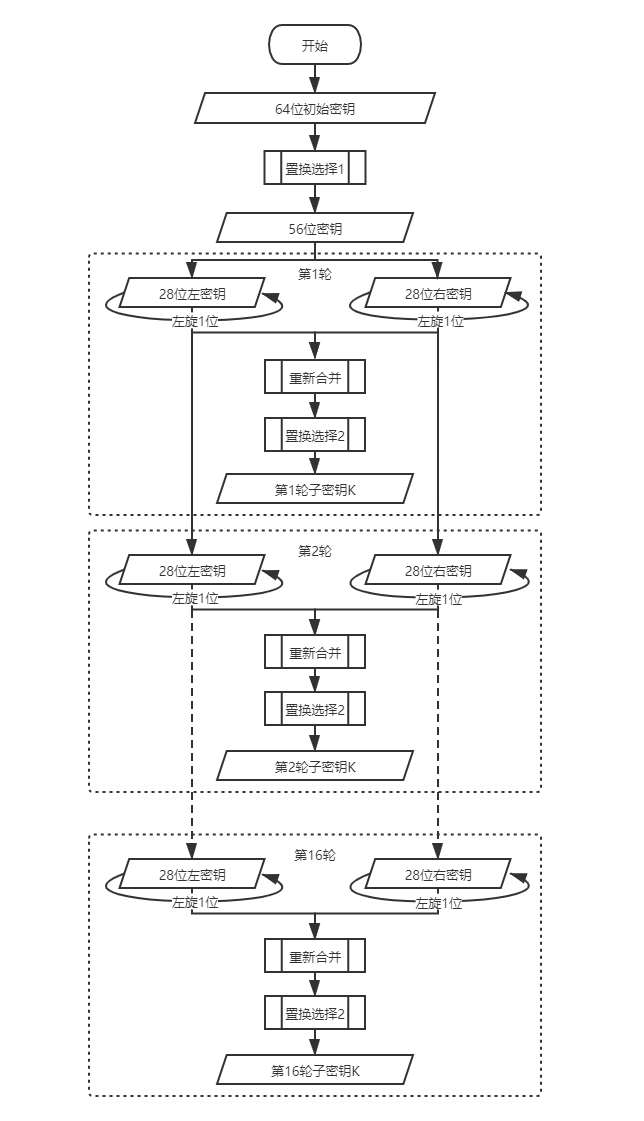
\includegraphics[width=0.82\textwidth]{my密钥流程图.png}
                    \caption{子密钥生成流程图}
                    \label{fig:key_gen_flow}
                \end{figure}
                伪代码如算法\ref{alg:key_generator}所示。
                \begin{algorithm}[htbp]
                    \caption{子密钥生成}
                    \label{alg:key_generator}
                    \begin{algorithmic}[1]
                        \Require 64位密钥$key$
                        \Ensure $K$数组
                        \Function{KeyGen}{$key$}
							\State $init\_key\gets key\_transform(key)$;
							\State $L\_key,R\_key\gets key\_split(init\_key)$;
							\State $rot\_table\gets [1, 1, 2, 2, 2, 2, 2, 2, 1, 2, 2, 2, 2, 2, 2, 1]$
							\For{$i=1\to16$}
								\State $left\_rot(L\_key,rot\_table[i])$;
								\State $left\_rot(R\_key,rot\_table[i])$;
								\State $merge\_key \gets merge(L\_key, R\_key)$;
								\State $K[i]\gets key\_sepermuted(merge\_key)$;
							\EndFor
							\State \Return{$K$}
                        \EndFunction
                    \end{algorithmic}
                \end{algorithm}
                \par 由上述流程图与伪代码对算法的描述可知,子密钥生成部分需要调用的函数有初始密钥转换函数,左右密钥分离函数,密钥合并函数和密钥置换选择函数。
                \paragraph{置换函数} DES中,置换的功能是将输入的数据按位以某一特定规律重新组合。
                \par 由于DES算法中,大部分置换的原理相同,都是将某一位的二进制数据根据表格移动到另一个位置,因此可以最终都引用到同一个函数。所有的置换步骤只需要提供置换表格并调用这个函数即可完成。
                \par 该函数的伪代码如\cref{alg:transform}所示。
                \begin{algorithm}[htbp]
                	\caption{置换函数}
                	\label{alg:transform}
                	\begin{algorithmic}[1]
                		\Require 置换前的$input$,置换表$table$
                		\Ensure 置换后的$output$
                		\Function{Transform}{$input$, $table$}
                		\State $output \gets 0$;
                		\For{$i=1\to length(table)$}
							\State $output \gets output\ll 1$;
							\State $output \gets output\ |\ ((input \gg (length(input) - table[i]))\ \&\ 1)$;
				  		\EndFor
                		\State \Return{$output$}
                		\EndFunction
                	\end{algorithmic}
                \end{algorithm}
            	\par 为了起到加快运算速度的效果,在DES算法的书写时,考虑直接使用二进制位运算进行。由于实现算法时,为节省空间,全程使用了整型以保存密钥及名密文,因此在编写程序进行运算时,需要注意(以bit为单位的)大小端的问题。
            	\paragraph{密钥初始置换} 此函数删除密钥奇偶校验位,将64位密钥变为56位。实现时只需要提供置换表并调用置换函数即可。
            	\paragraph{左右拆分} 由于在加解密过程与密钥生成过程都用到了这一个函数,为确保代码简洁性,将其单独作为一个函数。同样采用位运算以加快程序速度,伪代码如\cref{alg:split}所示。
            	\begin{algorithm}[htbp]
            		\caption{左右拆分}
            		\label{alg:split}
            		\begin{algorithmic}[1]
            			\Require 拆分前的$input$
            			\Ensure 拆分后的$left, right$
            			\Function{Split}{$input$}
            			\State $left \gets input\gg(length(input) / 2)$;
            			\State $right \gets input\ \mod (1\ll length(input) / 2)$;
            			\State \Return{$left, right$}
            			\EndFunction
            		\end{algorithmic}
            	\end{algorithm}
            	\paragraph{密钥左旋} 算法采用位运算,输入密钥、长度与密钥左旋的位数,返回左旋结果。具体实现如\cref{alg:LeftRot}所示。
            	\begin{algorithm}[htbp]
            		\caption{密钥左旋}
            		\label{alg:LeftRot}
            		\begin{algorithmic}[1]
            			\Require 左旋前的$input$,左旋轮数$round$
            			\Ensure 左旋后的$output$
            			\Function{LeftRot}{$input$, $round$}
            			\State $input \gets input\ll round$;
            			\State $output \gets input\ |\ (input\gg length(input))$;
            			\State $output \gets output\mod (1\ll length(input))$;
            			\State \Return{$output$}
            			\EndFunction
            		\end{algorithmic}
            	\end{algorithm}
            	\paragraph{合并函数} 合并函数将左右两部分合并。具体实现如\cref{alg:merge}所示。
            	\begin{algorithm}[htbp]
            		\caption{合并函数}
            		\label{alg:merge}
            		\begin{algorithmic}[1]
            			\Require $left, right$
            			\Ensure $output$
            			\Function{Merge}{$left$, $right$}
            			\State $output\gets (left\ll lenght(right)) + right$;
            			\State \Return{$output$}
            			\EndFunction
            		\end{algorithmic}
            	\end{algorithm}
            	\paragraph{密钥置换选择} 此函数与此节的密钥初始置换相似,提供置换表格并调用置换函数即可。
            \subsubsection{加密和解密}
                加密与解密算法流程图如\cref{fig:crypt_flow}所示。
                \begin{figure}[htbp]
                    \centering
                    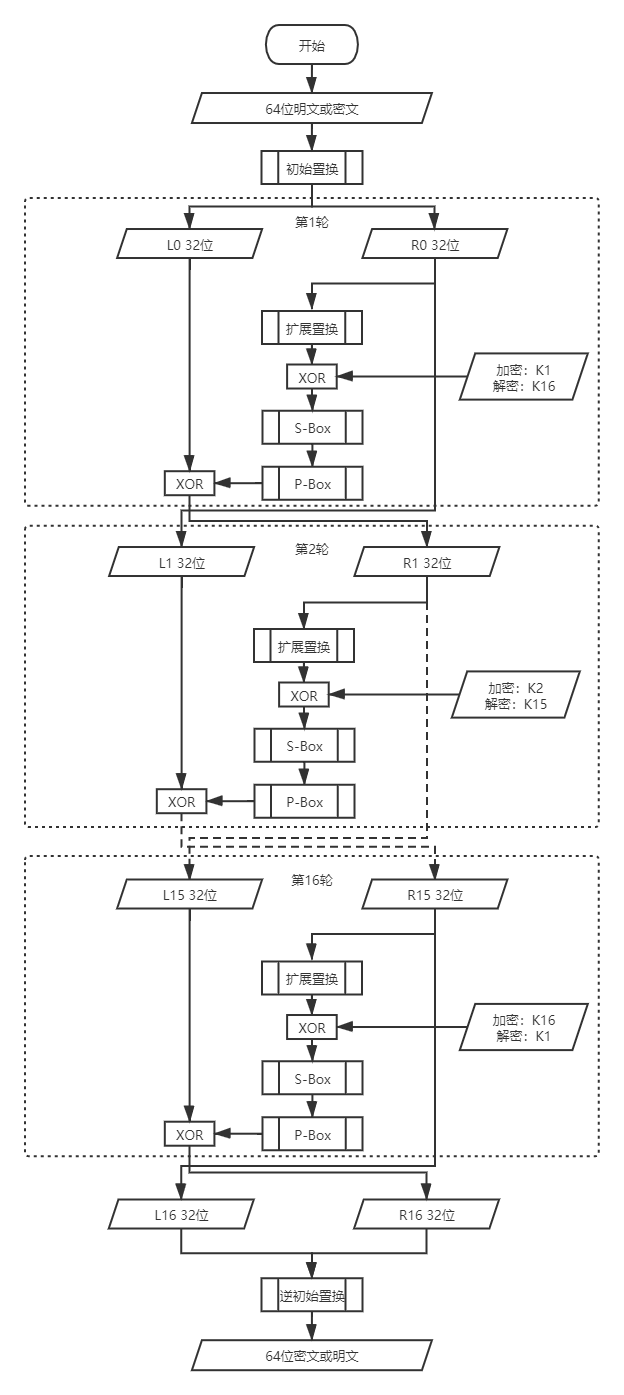
\includegraphics[width=0.65\textwidth]{my加解密流程图.png}
                    \caption{加密解密流程图}
                    \label{fig:crypt_flow}
                \end{figure}
            	伪代码如\cref{alg:crypt_algorithm}所示。解密时反向使用16个子密钥即可。
            	\begin{algorithm}[htbp]
            		\caption{加密解密算法}
            		\label{alg:crypt_algorithm}
            		\begin{algorithmic}[1]
            			\Require 64位明文或密文$text$,64位密钥$key$
            			\Ensure 64位密文或明文$output$
            			\Function{KeyGen}{$key$}
            			\State $init\_K\gets des\_key\_create(key)$;
            			\State $init\_text\gets des\_initial(text)$;
            			\State $L\_text,R\_text\gets text\_split(init\_text)$;
            			\For{$i=1\to16$}
            				\State $L\_text, R\_text\gets des_calc(L\_text,R\_text,K[i])$;
            			\EndFor
            			\State $L\_text, R\_text\gets R\_text, L\_text$;
            			\State $output \gets merge(L\_text,R\_text)$;
            			\State $output \gets final\_transform(output)$;
            			\State \Return{$output$}
            			\EndFunction
            		\end{algorithmic}
            	\end{algorithm}
            	\par 由上述流程图与代码对算法的描述可知,加解密部分需要调用的函数有初始置换,左右分离函数,扩展置换函数,S盒函数,P盒函数,合并函数和逆初始置换函数。
            	\paragraph{初始置换,扩展至换,P盒,逆初始置换} 加密算法中需要使用的四个置换函数原理与密钥生成部分中的置换函数原理相同,提供置换表并调用置换函数即可,代码简单,此处不再列出。
            	\paragraph{S盒函数} DES算法的S盒函数,是将六位输入映射到四位输出上,S盒子由8个4行16列的表格构成。算法首先将48位输入拆分为8组,每一组使用一个S盒,使用时,选择六位输入的第一位与最后一位决定行,中间四位决定列,最终映射到的数据就是用来替换的数据,最后将8个4比特数据合并,得到32位输出。具体实现如\cref{alg:dessbox}所示。
            	\begin{algorithm}[htbp]
            		\caption{SBOX函数}
            		\label{alg:dessbox}
            		\begin{algorithmic}[1]
            			\Require 置换前的$input$,$SBOX$
            			\Ensure 置换后的$output$
            			\Function{SBOX}{$input, SBOX$}
            			\State $output \gets 0$;
            			\For{$i=1\to 8$}
            				\State $output \gets output \ll 4$;
            				\State $tmp = (input\gg (48-6\times(i+1)))\ \&\ 3fh$;
            				\State $tmp = (tmp\ \&\ 20h) + ((tmp\ \&\ 1) \ll 4)+((tmp\ \&\ 1eh)\gg 1)$;
            				\State $output \gets output + SBOX[i][tmp]$;
            			\EndFor
            			\State \Return{$output$}
            			\EndFunction
            		\end{algorithmic}
            	\end{algorithm}
				\par 其余函数在上一节中均已有过讲述,此处省略。
            \subsection{算法优化}
            	\subsubsection{速度优化} DES算法中引入了大量的移位操作,因此,使用数组进行运算更加直观。然而数组运算将会造成大量的空间开销,在时间上也不是最优方案,如果采用整型对数据进行存储,则可以用位运算与赋值语句代替移位操作,并增大信息存储的密度,从而起到减小时间开销与空间开销的效果\upcite{1}。由于代码最开始便采用了整型作为数据存储类型,因此此步优化效果已经达成。
            	\par 除了数据类型上的优化之外,算法本身也可以进行优化。观察发现,在DES算法中,部分置换函数可以整合在一起或者进行简化。如加解密算法中的扩展置换函数,其置换表格具有较强的规律性,完全可以利用位运算实现\upcite{1}。具体代码如\cref{alg:fastexpansion}所示。
				\begin{algorithm}[htbp]
            		\caption{快速扩展置换}
            		\label{alg:fastexpansion}
            		\begin{algorithmic}[1]
            			\Require 32位$input$
            			\Ensure 48位$output$
            			\Function{FastExpension}{$input$}
            			\State $output\gets input\ \&\ 1$;
            			\State $output = (output \ll 5)\ |\ ((input \gg 27)\ \&\ 1fh)$;
            			\State $output = (output \ll 6)\ |\ ((input \gg 23)\ \&\ 3fh)$;
            			\State $output = (output \ll 6)\ |\ ((input \gg 19)\ \&\ 3fh)$;
            			\State $output = (output \ll 6)\ |\ ((input \gg 15)\ \&\ 3fh)$;
            			\State $output = (output \ll 6)\ |\ ((input \gg 11)\ \&\ 3fh)$;
            			\State $output = (output \ll 6)\ |\ ((input \gg  7)\ \&\ 3fh)$;
            			\State $output = (output \ll 6)\ |\ ((input \gg  3)\ \&\ 3fh)$;
            			\State $output = (output \ll 5)\ |\ (input\ \&\ 1fh)$;
            			\State $output = (output \ll 1)\ |\ ((input \gg 31)\ \&\ 1)$;
            			\State \Return{$output$}
            			\EndFunction
            		\end{algorithmic}
            	\end{algorithm}
				\par 而对于置换函数的优化,观察发现,S盒函数在使用时相当于调用了另一个经过简单移位后的S盒,因此可以重新构造S盒,使得对于任意的输入,可以直接通过地址来获得输出,而无需再进行位运算。同时,可以将S盒运算后的结果直接再进行一个P盒映射,多个映射的结果可以由拼接改为异或运算,这一步在整型数据结构中实现较为容易,并可以省去一个P盒置换的时间,加快运算速度\upcite{1,2}。将两个优化方案结合后的代码如\cref{alg:fastpsbox}所示,具体的PS盒内容见\cref{apx:spbox}。
				\begin{algorithm}[htbp]
					\caption{SBOX函数}
					\label{alg:fastpsbox}
					\begin{algorithmic}[1]
						\Require 置换前的$input$,$PSBOX$
						\Ensure 置换后的$output$
						\Function{SBOX}{$input, PSBOX$}
						\State $output \gets 0$;
						\For{$i=1\to 8$}
						\State $tmp = (input\gg (48-6\times i))\ \&\ 3fh$;
						\State $output \gets output + PSBOX[i][tmp]$;
						\EndFor
						\State \Return{$output$}
						\EndFunction
					\end{algorithmic}
				\end{algorithm}
				\subsubsection{安全性优化}
					在算法安全性上,可以通过增加密钥的实际使用长度来增加算法的随机性,以此抵御线性逼近攻击、差分攻击等攻击方式。在常规的DES算法中,SBOX的使用顺序是固定的,而将被抛弃的密钥可以利用排列组合来更改SBOX的顺序,由原先的一种SBOX模式扩展为 $8!$ 种模式\upcite{3}。
					\par 其具体操作方式为\upcite{4}:
					\begin{enumerate}[1.]
						\item 将8位被丢弃的密钥位连接,整合为一个二进制数字 $H$。
						\item 由于8个SBOX共有$8!$种排列方式,因此计算对$R=H\mod{8!}$。
						\item 由组合数学可以算出 $H=R_7\cdot 7!+R_6\cdot 6!+R_5\cdot 5!+R_4\cdot 4!+R_3\cdot 3!+R_2\cdot 2!+R_1$。
						\item 由$(R_7,R_6,R_5,R_4,R_3,R_2,R_1)$可以生成一个$1,2\ldots,8$的一个排列,其中 $R_7$ 表示SBOX8右边有几个S盒子的序号比它小,$R_6\ldots R_1$同理。
					\end{enumerate}
					\par 然而这样的操作仍有一些潜在的问题,其选择的8位弃置密钥最多只含有$8\mathrm{bit}$的信息量,而所有的排列有$\log_2 8!\approx15.2\mathrm{bit}$的信息量,即,在八位密钥下,$H$远小于$8!$,无法提供足够的SBOX排列方案。因此,要想更好的进行SBOX的随机化,可以将所有抛弃的密钥位置合并使用,每一轮中使用16位弃置的密钥进行计算,这样可以确保每种排列方式均有可能被使用。在具体操作上,由于初始置换中抛弃的密钥是固定的,应选择将其作为$H$的后八位,以增大SBOX的随机性。由于该优化核心为数学原理,部分代码在\cref{apx:safety}中给出。
		\subsection{测试样例与结果截图}
			测试样例如\cref{apx:testcode}中的\cref{lst:destest}所示。
			\par 结果截图如\cref{fig:destestres}所示。
			\begin{figure}[htbp]
				\centering
				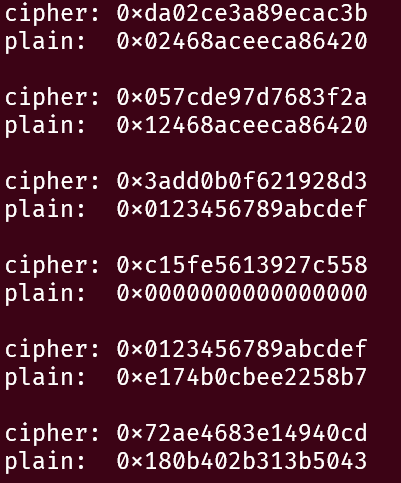
\includegraphics{des_test_res.png}
				\caption{DES算法测试数据结果截图}
				\label{fig:destestres}
			\end{figure}
			\par 优化效果的测试样例如\cref{apx:testcode}中的\cref{lst:desspeedcmp}所示。测试平台:i5-7200U,WSL Ubuntu,python3.6.9。

			测试结果如\cref{fig:destestspeed}所示。前两行为优化后与优化前计算1000次的时间,最后一行为优化倍数。
			\begin{figure}[htbp]
				\centering
				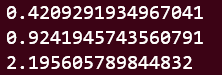
\includegraphics{优化结果.png}
				\caption{DES算法优化效果测试结果截图}
				\label{fig:destestspeed}
			\end{figure}
		\section{收获与建议}
		在本次实验中,主要进行了DES算法的实现与优化。由于DES算法相较于AES等算法来说较为简单,且数学原理较少,因此非常适合用于巩固自己的分组密码基础,也能够更好的体会Feistal密码体系。除此之外,考虑到未来实验的命名空间问题,在大部分的函数名称中加入了des的前缀,为解决这个问题,发现可以在名称前加入两个下划线,以此成为私有方法,可以很好地解决命名空间的问题,在此后的实验中会对此进行尝试。
		\par 在根据论文进行算法安全性优化时,发现论文中在某些细节上存在问题,因此对其进行修正后进行使用,但由于没有相应的测试数据,因此无法对正确性进行充分的判断,但可以确定以同样的方式进行解密后的结果与明文相同。
		\par 进行速度优化时,由于最开始进行实验时就采用了整型数据结构进行存储与计算,因此后续只能对PSBOX以及扩展置换等地方进行优化,优化结果仅能做到效率翻倍,效果不如论文中的明显。
		\par 在本次实验中,直到助教提醒前并未在文档中发现思考题,建议在实验指导书中,将思考题部分放到实验报告要求之前。
		\par 完成本次实验后,认为在流程图上消耗了大量精力,由于DES整体的算法都是通过他人的流程图与解释进行学习的,因此在自己绘制流程图时,往往会与他人的流程图较为相似。从这一角度来看,绘制流程图这一步骤浪费了大量时间,且收获较小,希望可以直接引用经典且开源的流程图,这样既可以做到清晰美观,又可以尽可能避免重复他人操作。此外,在DES密码算法以及后续的分组密码算法中,核心的流程图可以很清晰的显示出函数调用,而且在实际算法分析时,函数调用图极少使用,从这一点来看,进行函数调用图的绘制是没有必要的。
    \begin{thebibliography}{99}
    	\bibitem{1}
		郑焰.DES算法软件速度优化的实现[J].计算机安全,2005(08):21-23.
		\bibitem{2}
		陈良.一种优化DES算法[J].计算机工程与应用,2004(06):74-76+86.
		\bibitem{3}
		付秀伟.基于DES算法的系统优化设计[J].吉林化工学院学报,2012,29(11):127-129.
		\bibitem{4}
		肖堃,罗蕾.一种DES的改进方案[J].福建电脑,2008(05):77-78.
	\end{thebibliography}
	\newpage
	\appendix
	\section{结果测试代码}\label{apx:testcode}
	\begin{lstlisting}[caption={des\_test}, label={lst:destest}]
import CNSPP
		
test_unsafe_des = [
	[0x02468aceeca86420, 0x0f1571c947d9e859],
	[0x12468aceeca86420, 0x0f1571c947d9e859],
	[0x0123456789abcdef, 0x1f1571c947d9e859],
	[0x0000000000000000, 0x3abb72cbe0204027],
	[0xe174b0cbee2258b7, 0xbcca87bb9320ef40],
	[0x180b402b313b5043, 0xda8483580415016b]
]
		
for test in test_unsafe_des:
	cipher = CNSPP.des_encrypt(test[0], test[1])
	print ('cipher:', end = ' ')
	CNSPP.print_hex_as_len(cipher, 16)
	print ('plain:', end = '  ')
	CNSPP.print_hex_as_len(CNSPP.des_decrypt(cipher, test[1]), 16)
	print ()
	\end{lstlisting}
	\begin{lstlisting}[caption={des\_speed\_cmp}, label={lst:desspeedcmp}]
import CNSPP			
import time
	
t0 = time.time()
for i in range(1000):
	CNSPP.des_encrypt(0x0123456789ABCDEF, 0x133457799BBCDFF1)
t0 = time.time() - t0
print (t0)
	
t1 = time.time()
for i in range(1000):
	CNSPP.des_std_encrypt(0x0123456789ABCDEF, 0x133457799BBCDFF1)
t1 = time.time() - t1
print (t1)
print (t1 / t0)
	\end{lstlisting}
	\section{思考题}
	\subsection{针对DES密码分析的成果}
	DES加密算法曾是最为流行的加密算法之一,因此早期的密码分析大多针对DES算法进行。到90年代,研究出了两个重要的成果——差分密码分析和线性密码分析,而这两种方法也是攻击迭代密码最为有效的方法之一。其中差分攻击更加有效,除DES算法外,对同为SPN网络的AES算法和SM4算法也可以进行攻击。差分分析本质上属于选择明文攻击,通过寻找具有某些特定差分的明密文对,并进行比较,可以计算出密钥的概率值。
	\par 差分攻击针对缺少高概率差分特征的分组密码效果较差,因此在此基础上研究出了针对DES的截断差分分析方法,可以以更低的复杂度进行攻击,得以广泛应用。
	\subsection{DES算法不适用于现代的原因}
	DES算法已经被确定为不安全的密码,主要原因在于其密钥过短,仅仅有56位,因此在计算机的算力大幅度提高后,其被破解的速度越来越快。
	\par 在1999年,DES在22小时15分钟内被破解。到了2007年,一台1万美金的电脑平均6.4天即可破解DES。到2016年,开源软件hashcat在通用GPU上加入了DES暴力破解功能,使用1080Ti显卡,平均15天就能恢复一个密钥。到2017年,使用rainbow table的选择明文攻击可以在25秒内破解一个DES算法的密钥,对于每个明文,需要使用一个新的rainbow table,而网络上已经可以下载到一些rainbow table。
	\par 以上各个数据均表明,随着计算机硬件的发展,计算机计算速度的提高,密钥长度较短的DES算法已经无法满足加密的需要。因此不适用于现代。
	\section{安全性优化部分代码}\label{apx:safety}
	\par SBOX安全性优化的部分代码如\cref{safetysbox}所示。其中,order数组保存的就是重新排列后SBOX的顺序。
	\begin{lstlisting}[caption={safty\_SBOX}, label={safetysbox}]
H = ab_key % 40320
R = [0] * 7
modulo = 5040
for i in range(7):
	R[6 - i] = H // modulo
	H %= modulo
	modulo //= (7 - i)
order = [0] * 8
for i in range(6, -1, -1):
	place = 7
	for j in range(R[i]):
		while order[place] != 0:
			place -= 1
		place -= 1
	while order[place] != 0:
		place -= 1
	order[place] = i + 1
	\end{lstlisting}
	\par 同时,需要在密钥生成过程中,保存被抛弃的密钥,因此密钥生成算法的过程修改结果如\cref{newdeskeycreate}所示。
	\begin{lstlisting}[caption={des\_key\_create}, label={newdeskeycreate}]
def des_key_create(raw_key):
	raw_key, init_abandon = des_key_init_transform(raw_key)
	raw_key = half_split(raw_key, 56)
	key_left_rot_table = [1, 1, 2, 2, 2, 2, 2, 2, 1, 2, 2, 2, 2, 2, 2, 1]
	key = []
	ab_key = []
	for round in range(16):
		raw_key[0] = left_rot(raw_key[0], 28, key_left_rot_table[round])
		raw_key[1] = left_rot(raw_key[1], 28, key_left_rot_table[round])
		new_key, abandon_key = des_sepermuted(re_merge(raw_key, 28))
		key.append(new_key)
	ab_key.append(abandon_key << 8 | init_abandon)
	return key, ab_key
	\end{lstlisting}
	\section{附录:速度优化后的PS盒具体数据}\label{apx:spbox}
	具体数据如\cref{table:PSBox-1,table:PSBox-2,table:PSBox-3,table:PSBox-4,table:PSBox-5,table:PSBox-6,table:PSBox-7,table:PSBox-8}所示。由于算法采用整型数据进行实现,此处需要注意大小端(这里指以bit为单位的大小端)问题。如文献\upcite{2}中所提供的PSBOX,就与实际使用时所需的PSBOX并不相同,需要进行按位反转方能使用。
	\begin{table}[htbp]
		\caption{PSBox-1}
		\label{table:PSBox-1}
		\centering
		\setlength{\tabcolsep}{1mm}{\begin{tabular}{cccccccc}
			\hline
			0x00808200 & 0x00000000 & 0x00008000 & 0x00808202 \\ 
			0x00808002 & 0x00008202 & 0x00000002 & 0x00008000 \\ 
			0x00000200 & 0x00808200 & 0x00808202 & 0x00000200 \\ 
			0x00800202 & 0x00808002 & 0x00800000 & 0x00000002 \\ 
			0x00000202 & 0x00800200 & 0x00800200 & 0x00008200 \\ 
			0x00008200 & 0x00808000 & 0x00808000 & 0x00800202 \\ 
			0x00008002 & 0x00800002 & 0x00800002 & 0x00008002 \\ 
			0x00000000 & 0x00000202 & 0x00008202 & 0x00800000 \\ 
			0x00008000 & 0x00808202 & 0x00000002 & 0x00808000 \\ 
			0x00808200 & 0x00800000 & 0x00800000 & 0x00000200 \\ 
			0x00808002 & 0x00008000 & 0x00008200 & 0x00800002 \\ 
			0x00000200 & 0x00000002 & 0x00800202 & 0x00008202 \\ 
			0x00808202 & 0x00008002 & 0x00808000 & 0x00800202 \\ 
			0x00800002 & 0x00000202 & 0x00008202 & 0x00808200 \\ 
			0x00000202 & 0x00800200 & 0x00800200 & 0x00000000 \\ 
			0x00008002 & 0x00008200 & 0x00000000 & 0x00808002 \\
			\hline
		\end{tabular}}
	\end{table}
	\begin{table}[htbp]
		\caption{PSBox-2}
		\label{table:PSBox-2}
		\centering
		\setlength{\tabcolsep}{1mm}{\begin{tabular}{cccccccc}
			\hline
			0x40084010 & 0x40004000 & 0x00004000 & 0x00084010 \\
			0x00080000 & 0x00000010 & 0x40080010 & 0x40004010 \\
			0x40000010 & 0x40084010 & 0x40084000 & 0x40000000 \\
			0x40004000 & 0x00080000 & 0x00000010 & 0x40080010 \\
			0x00084000 & 0x00080010 & 0x40004010 & 0x00000000 \\
			0x40000000 & 0x00004000 & 0x00084010 & 0x40080000 \\
			0x00080010 & 0x40000010 & 0x00000000 & 0x00084000 \\
			0x00004010 & 0x40084000 & 0x40080000 & 0x00004010 \\
			0x00000000 & 0x00084010 & 0x40080010 & 0x00080000 \\
			0x40004010 & 0x40080000 & 0x40084000 & 0x00004000 \\
			0x40080000 & 0x40004000 & 0x00000010 & 0x40084010 \\
			0x00084010 & 0x00000010 & 0x00004000 & 0x40000000 \\
			0x00004010 & 0x40084000 & 0x00080000 & 0x40000010 \\
			0x00080010 & 0x40004010 & 0x40000010 & 0x00080010 \\
			0x00084000 & 0x00000000 & 0x40004000 & 0x00004010 \\
			0x40000000 & 0x40080010 & 0x40084010 & 0x00084000 \\
			\hline
		\end{tabular}}
	\end{table}
	\begin{table}[htbp]
		\caption{PSBox-3}
		\label{table:PSBox-3}
		\centering
		\setlength{\tabcolsep}{1mm}{\begin{tabular}{cccccccc}
			\hline
			0x00000104 & 0x04010100 & 0x00000000 & 0x04010004 \\ 
			0x04000100 & 0x00000000 & 0x00010104 & 0x04000100 \\ 
			0x00010004 & 0x04000004 & 0x04000004 & 0x00010000 \\ 
			0x04010104 & 0x00010004 & 0x04010000 & 0x00000104 \\ 
			0x04000000 & 0x00000004 & 0x04010100 & 0x00000100 \\ 
			0x00010100 & 0x04010000 & 0x04010004 & 0x00010104 \\ 
			0x04000104 & 0x00010100 & 0x00010000 & 0x04000104 \\ 
			0x00000004 & 0x04010104 & 0x00000100 & 0x04000000 \\ 
			0x04010100 & 0x04000000 & 0x00010004 & 0x00000104 \\ 
			0x00010000 & 0x04010100 & 0x04000100 & 0x00000000 \\ 
			0x00000100 & 0x00010004 & 0x04010104 & 0x04000100 \\ 
			0x04000004 & 0x00000100 & 0x00000000 & 0x04010004 \\ 
			0x04000104 & 0x00010000 & 0x04000000 & 0x04010104 \\ 
			0x00000004 & 0x00010104 & 0x00010100 & 0x04000004 \\ 
			0x04010000 & 0x04000104 & 0x00000104 & 0x04010000 \\ 
			0x00010104 & 0x00000004 & 0x04010004 & 0x00010100 \\
			\hline
		\end{tabular}}
	\end{table}
	\begin{table}[htbp]
		\caption{PSBox-4}
		\label{table:PSBox-4}
		\centering
		\setlength{\tabcolsep}{1mm}{\begin{tabular}{cccccccc}
			\hline
			0x80401000 & 0x80001040 & 0x80001040 & 0x00000040 \\ 
			0x00401040 & 0x80400040 & 0x80400000 & 0x80001000 \\ 
			0x00000000 & 0x00401000 & 0x00401000 & 0x80401040 \\ 
			0x80000040 & 0x00000000 & 0x00400040 & 0x80400000 \\ 
			0x80000000 & 0x00001000 & 0x00400000 & 0x80401000 \\ 
			0x00000040 & 0x00400000 & 0x80001000 & 0x00001040 \\ 
			0x80400040 & 0x80000000 & 0x00001040 & 0x00400040 \\ 
			0x00001000 & 0x00401040 & 0x80401040 & 0x80000040 \\ 
			0x00400040 & 0x80400000 & 0x00401000 & 0x80401040 \\ 
			0x80000040 & 0x00000000 & 0x00000000 & 0x00401000 \\ 
			0x00001040 & 0x00400040 & 0x80400040 & 0x80000000 \\ 
			0x80401000 & 0x80001040 & 0x80001040 & 0x00000040 \\ 
			0x80401040 & 0x80000040 & 0x80000000 & 0x00001000 \\ 
			0x80400000 & 0x80001000 & 0x00401040 & 0x80400040 \\ 
			0x80001000 & 0x00001040 & 0x00400000 & 0x80401000 \\ 
			0x00000040 & 0x00400000 & 0x00001000 & 0x00401040 \\
			\hline
		\end{tabular}}
	\end{table}
	\begin{table}[htbp]
		\caption{PSBox-5}
		\label{table:PSBox-5}
		\centering
		\setlength{\tabcolsep}{1mm}{\begin{tabular}{cccccccc}
			\hline
			0x00000080 & 0x01040080 & 0x01040000 & 0x21000080 \\
			0x00040000 & 0x00000080 & 0x20000000 & 0x01040000 \\
			0x20040080 & 0x00040000 & 0x01000080 & 0x20040080 \\
			0x21000080 & 0x21040000 & 0x00040080 & 0x20000000 \\
			0x01000000 & 0x20040000 & 0x20040000 & 0x00000000 \\
			0x20000080 & 0x21040080 & 0x21040080 & 0x01000080 \\
			0x21040000 & 0x20000080 & 0x00000000 & 0x21000000 \\
			0x01040080 & 0x01000000 & 0x21000000 & 0x00040080 \\
			0x00040000 & 0x21000080 & 0x00000080 & 0x01000000 \\
			0x20000000 & 0x01040000 & 0x21000080 & 0x20040080 \\
			0x01000080 & 0x20000000 & 0x21040000 & 0x01040080 \\
			0x20040080 & 0x00000080 & 0x01000000 & 0x21040000 \\
			0x21040080 & 0x00040080 & 0x21000000 & 0x21040080 \\
			0x01040000 & 0x00000000 & 0x20040000 & 0x21000000 \\
			0x00040080 & 0x01000080 & 0x20000080 & 0x00040000 \\
			0x00000000 & 0x20040000 & 0x01040080 & 0x20000080 \\
			\hline
		\end{tabular}}
	\end{table}
	\begin{table}[htbp]
		\caption{PSBox-6}
		\label{table:PSBox-6}
		\centering
		\setlength{\tabcolsep}{1mm}{\begin{tabular}{cccccccc}
			\hline
			0x10000008 & 0x10200000 & 0x00002000 & 0x10202008 \\
			0x10200000 & 0x00000008 & 0x10202008 & 0x00200000 \\
			0x10002000 & 0x00202008 & 0x00200000 & 0x10000008 \\
			0x00200008 & 0x10002000 & 0x10000000 & 0x00002008 \\
			0x00000000 & 0x00200008 & 0x10002008 & 0x00002000 \\
			0x00202000 & 0x10002008 & 0x00000008 & 0x10200008 \\
			0x10200008 & 0x00000000 & 0x00202008 & 0x10202000 \\
			0x00002008 & 0x00202000 & 0x10202000 & 0x10000000 \\
			0x10002000 & 0x00000008 & 0x10200008 & 0x00202000 \\
			0x10202008 & 0x00200000 & 0x00002008 & 0x10000008 \\
			0x00200000 & 0x10002000 & 0x10000000 & 0x00002008 \\
			0x10000008 & 0x10202008 & 0x00202000 & 0x10200000 \\
			0x00202008 & 0x10202000 & 0x00000000 & 0x10200008 \\
			0x00000008 & 0x00002000 & 0x10200000 & 0x00202008 \\
			0x00002000 & 0x00200008 & 0x10002008 & 0x00000000 \\
			0x10202000 & 0x10000000 & 0x00200008 & 0x10002008 \\
			\hline
		\end{tabular}}
	\end{table}
	\begin{table}[htbp]
		\caption{PSBox-7}
		\label{table:PSBox-7}
		\centering
		\setlength{\tabcolsep}{1mm}{\begin{tabular}{cccccccc}
			\hline
			0x00100000 & 0x02100001 & 0x02000401 & 0x00000000 \\
			0x00000400 & 0x02000401 & 0x00100401 & 0x02100400 \\
			0x02100401 & 0x00100000 & 0x00000000 & 0x02000001 \\
			0x00000001 & 0x02000000 & 0x02100001 & 0x00000401 \\
			0x02000400 & 0x00100401 & 0x00100001 & 0x02000400 \\
			0x02000001 & 0x02100000 & 0x02100400 & 0x00100001 \\
			0x02100000 & 0x00000400 & 0x00000401 & 0x02100401 \\
			0x00100400 & 0x00000001 & 0x02000000 & 0x00100400 \\
			0x02000000 & 0x00100400 & 0x00100000 & 0x02000401 \\
			0x02000401 & 0x02100001 & 0x02100001 & 0x00000001 \\
			0x00100001 & 0x02000000 & 0x02000400 & 0x00100000 \\
			0x02100400 & 0x00000401 & 0x00100401 & 0x02100400 \\
			0x00000401 & 0x02000001 & 0x02100401 & 0x02100000 \\
			0x00100400 & 0x00000000 & 0x00000001 & 0x02100401 \\
			0x00000000 & 0x00100401 & 0x02100000 & 0x00000400 \\
			0x02000001 & 0x02000400 & 0x00000400 & 0x00100001 \\
			\hline
		\end{tabular}}
	\end{table}
	\begin{table}[htbp]
		\caption{PSBox-8}
		\label{table:PSBox-8}
		\centering
		\setlength{\tabcolsep}{1mm}{\begin{tabular}{cccccccc}
			\hline
			0x08000820 & 0x00000800 & 0x00020000 & 0x08020820 \\
			0x08000000 & 0x08000820 & 0x00000020 & 0x08000000 \\
			0x00020020 & 0x08020000 & 0x08020820 & 0x00020800 \\
			0x08020800 & 0x00020820 & 0x00000800 & 0x00000020 \\
			0x08020000 & 0x08000020 & 0x08000800 & 0x00000820 \\
			0x00020800 & 0x00020020 & 0x08020020 & 0x08020800 \\
			0x00000820 & 0x00000000 & 0x00000000 & 0x08020020 \\
			0x08000020 & 0x08000800 & 0x00020820 & 0x00020000 \\
			0x00020820 & 0x00020000 & 0x08020800 & 0x00000800 \\
			0x00000020 & 0x08020020 & 0x00000800 & 0x00020820 \\
			0x08000800 & 0x00000020 & 0x08000020 & 0x08020000 \\
			0x08020020 & 0x08000000 & 0x00020000 & 0x08000820 \\
			0x00000000 & 0x08020820 & 0x00020020 & 0x08000020 \\
			0x08020000 & 0x08000800 & 0x08000820 & 0x00000000 \\
			0x08020820 & 0x00020800 & 0x00020800 & 0x00000820 \\
			0x00000820 & 0x00020020 & 0x08000000 & 0x08020800 \\
			\hline
		\end{tabular}}
	\end{table}
\end{document}